\section{Resultados}
\label{sec:resultados}

\begin{figure}[!t]
\centering
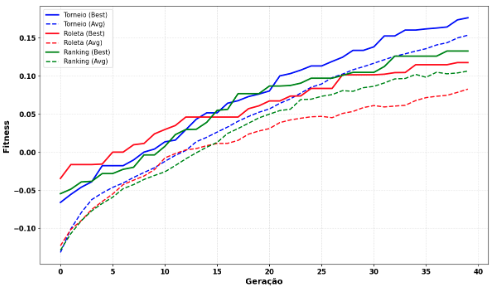
\includegraphics[width=\columnwidth]{selecao_colab}
\caption{Convergência por método de seleção, com uma execução por método: melhor aptidão (Best, linhas cheias) e aptidão média da população (Avg, tracejadas). O torneio é a configuração base.}
\label{fig:selecao}
\end{figure}

\begin{figure}[!t]
\centering
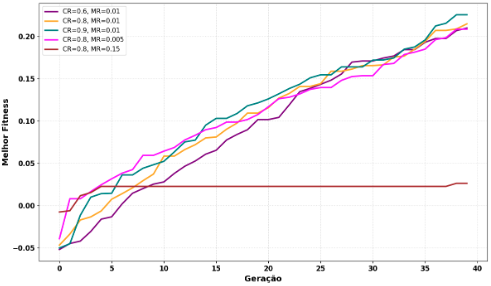
\includegraphics[width=\columnwidth]{taxas_colab}
\caption{Melhor aptidão por geração para as taxas de cruzamento (CR, $p_c$) e de mutação (MR, $p_m$), com uma execução por cenário. A configuração base é $p_c = 0,8$ e $p_m = 0,01$.}
\label{fig:taxas}
\end{figure}

\begin{figure}[!t]
\centering
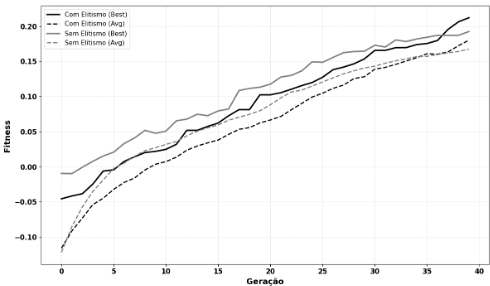
\includegraphics[width=\columnwidth]{elitismo_colab}
\caption{Convergência com e sem elitismo: melhor aptidão (Best, linhas cheias) e aptidão média da população (Avg, tracejadas).}
\label{fig:elitismo}
\end{figure}

\begin{table}[!t]
\caption{Aptidão do melhor indivíduo e média da população}
\label{tab:resultados}
\centering
\footnotesize
\begin{tabular}{@{}lccc@{}}
\toprule
Cenário & \begin{tabular}[c]{@{}c@{}}Melhor\\ger.~0\end{tabular} & \begin{tabular}[c]{@{}c@{}}Melhor\\ger.~39\end{tabular} & \begin{tabular}[c]{@{}c@{}}Média\\ger.~39\end{tabular} \\
\midrule
\multicolumn{4}{@{}l}{\textit{(a) Seleção}} \\
Roleta & $-0,034$ & 0,118 & 0,083 \\
Torneio$^{\dagger}$ & $-0,065$ & 0,177 & 0,150 \\
Ranking linear & $-0,054$ & 0,133 & 0,104 \\
\midrule
\multicolumn{4}{@{}l}{\textit{(b) Taxas}} \\
$p_c = 0,6$ & $-0,052$ & 0,210 & -- \\
$p_c = 0,8$, $p_m = 0,01^{\dagger}$ & $-0,046$ & 0,215 & -- \\
$p_c = 0,9$ & $-0,050$ & 0,226 & -- \\
$p_m = 0,005$ & $-0,037$ & 0,209 & -- \\
$p_m = 0,15$ & $-0,007$ & 0,026 & -- \\
\midrule
\multicolumn{4}{@{}l}{\textit{(c) Elitismo}} \\
Com elitismo$^{\dagger}$ & $-0,046$ & 0,212 & 0,180 \\
Sem elitismo & $-0,010$ & 0,192 & 0,167 \\
\bottomrule
\multicolumn{4}{@{}l}{\scriptsize $^{\dagger}$Configuração base. Valores de (a) e (b) lidos das curvas (precisão de $\pm 0,002$).}
\end{tabular}
\end{table}

As Figs.~\ref{fig:selecao} a~\ref{fig:elitismo} mostram as curvas de convergência, e a Tabela~\ref{tab:resultados}, a aptidão no início e no fim de cada execução. Como cada cenário foi executado uma única vez, parte das diferenças decorre da população inicial: a configuração base, presente nos três testes, terminou com melhor aptidão entre 0,177 e 0,215. Diferenças menores que cerca de 0,04 não podem, portanto, ser atribuídas com segurança à técnica.

Na seleção (Fig.~\ref{fig:selecao}), o torneio partiu da pior população inicial e terminou com a maior aptidão, tanto do melhor indivíduo (0,177, contra 0,133 do ranking e 0,118 da roleta) quanto da média da população (0,150, contra 0,104 e 0,083). Essa ordem coincide com a da pressão de seleção (Tabela~\ref{tab:selecao}). A roleta começou à frente, mas estagnou: nas últimas cinco gerações, seu melhor indivíduo melhorou 0,0006 por geração, contra 0,0033 no torneio.

Nas taxas (Fig.~\ref{fig:taxas}), $p_c$ = 0,6, 0,8 e 0,9 terminaram em 0,210, 0,215 e 0,226, e $p_m$ = 0,005, em 0,209: diferenças dentro da variação entre execuções, sem efeito conclusivo. Já $p_m$ = 0,15, que altera em média 105 genes por indivíduo, impediu a evolução: o melhor indivíduo ficou parado em 0,022 da 4.ª à 37.ª geração, sustentado apenas pelo elitismo, enquanto a aptidão média da população ficou em torno de $-0,05$.

Com elitismo (Fig.~\ref{fig:elitismo}), a melhor aptidão cresceu sem oscilações; sem elitismo, ela caiu sete vezes, ainda que pouco (no máximo 0,004). Mesmo partindo de uma população inicial pior ($-0,046$ contra $-0,010$), a execução com elitismo ultrapassou a outra na geração 37 e terminou à frente (0,212 contra 0,192).

Em todos os cenários, exceto $p_m$ = 0,15, as curvas ainda subiam na última geração, ou seja, 40 gerações não bastaram para a convergência. A melhor solução da execução com elitismo ($f = 0,212$) cobre 99,6\% da área de interesse com 228 passagens (32\% das candidatas), mas ainda com $\mathrm{SO} = 0,59$, o que indica redundância a eliminar.

Em síntese, entre os métodos de seleção, o torneio, de maior pressão de seleção, obteve a melhor aptidão; a taxa de mutação alta impediu a evolução; e o elitismo garantiu o crescimento sem oscilações da melhor aptidão. As variações de $p_c$ e as taxas de mutação baixas tiveram efeito menor que a variação entre execuções. Trabalhos futuros devem usar mais gerações e várias execuções por cenário, para confirmar estatisticamente essas diferenças.
